%!TEX root = ../../thesis.tex
\chapter{Modellierung und Implementation}
\label{cha:modelling}

Der zweite Teil der Arbeit beginnt mit einer Vorstellung des Entwicklungsprozesses des \textit{Garbage-Collection-Simulators}.
Nach einer kurzen Beschreibung der Anforderungen an diese Anwendung erfolgt ein Blick auf die Modellierung und Implementation der zentralen Programmkomponenten, wobei die wichtigsten Designentscheidungen erläutert werden.
Abschließend wird die Realisierung der grafischen Ausgabe erläutert, die für eine nachvollziehbare Darstellung der ausgewählten Algorithmen wesentlich ist.
Das folgende Kapitel beschreibt schließlich, wie die Anwendung zu verwenden ist und wie sie um weitere Algorithmen ergänzt werden kann.

\section{Spezifikation der Anforderungen}
\label{sec:requirements}
Der zu entwerfende Simulator soll die Ausführung ausgewählter Garbage-Collection-Algorithmen demonstrieren, sodass die einzelnen Arbeitsschritte eines Algorithmus klar erkennbar sind.
Dazu soll das in Kapitel~\ref{cha:intro} eingeführte Speichermodell realisiert werden.
Eine grafische Ausgabe visualisiert dabei den Heap als Blockgrafik: Belegte Teile des Heaps sollen von freien optisch unterschieden werden können, zudem sollen Lage und Größe der einzelnen Objekte erkennbar sein.
Die Anwenderin soll darüber hinaus die Möglichkeit haben, den Simulator zu konfigurieren:
Neben einer obligatorischen Auswahl des verwendeten Garbage-Collection-Algorithmus soll auch die Größe des Heaps sowie die Größe der erzeugten Heapobjekte einstellbar sein.
Weitere Anpassungsmöglichkeiten sind der Verzweigungsgrad der Objekte untereinander sowie die Verwaisungswahrscheinlichkeit, sodass verschiedene Objektkonstellationen betrachtet werden können.
Zuletzt soll durch eine Anpassbarkeit der Animationsgeschwindigkeit auch die Visualisierung konfigurierbar sein.

Aus Sicht der Softwareentwicklung ergeben sich zusätzliche Anforderungen, die für die Umsetzung der Anwendung relevant sind:
Der Simulator soll als frei verwendbare Software im Rahmen der Lehre eingesetzt werden können und beliebig anpassbar und erweiterbar sein, etwa indem Entwicklerinnen weitere Garbage-Collection-Algorithmen ergänzen.
Dies impliziert die Verwendung verschiedener Konzepte der Objektorientierung, unter anderem der Modularisierung in funktional unterscheidbare Pakete und Klassen, der Polymorphie und der generischen Programmierung.
Darüber hinaus soll die Anwendung plattformunabhängig entwickelt werden, um sie möglichst vielen Anwenderinnen zugänglich zu machen.

\section{Modellierung}
\label{sec:model}
Aufgrund der oben beschriebenen Anforderungen bietet sich die in Abbildung~\ref{fig:model} dargestellte Aufteilung in einzelne Komponenten an, auf deren Funktion im Folgenden eingegangen wird.
Bereits in Kapitel~\ref{cha:intro} wurde angemerkt, dass sich ein Programm grob in die drei Bestandteile Mutator, Allokator und Kollektor einteilen lässt.
Insofern ist es sinnvoll, diese Einteilung möglichst auch in die Modellierung einfließen zu lassen, insbesondere um verschiedene Kombinationen von Allokator und Kollektor zu ermöglichen.

\begin{figure}[h]
	\centering
	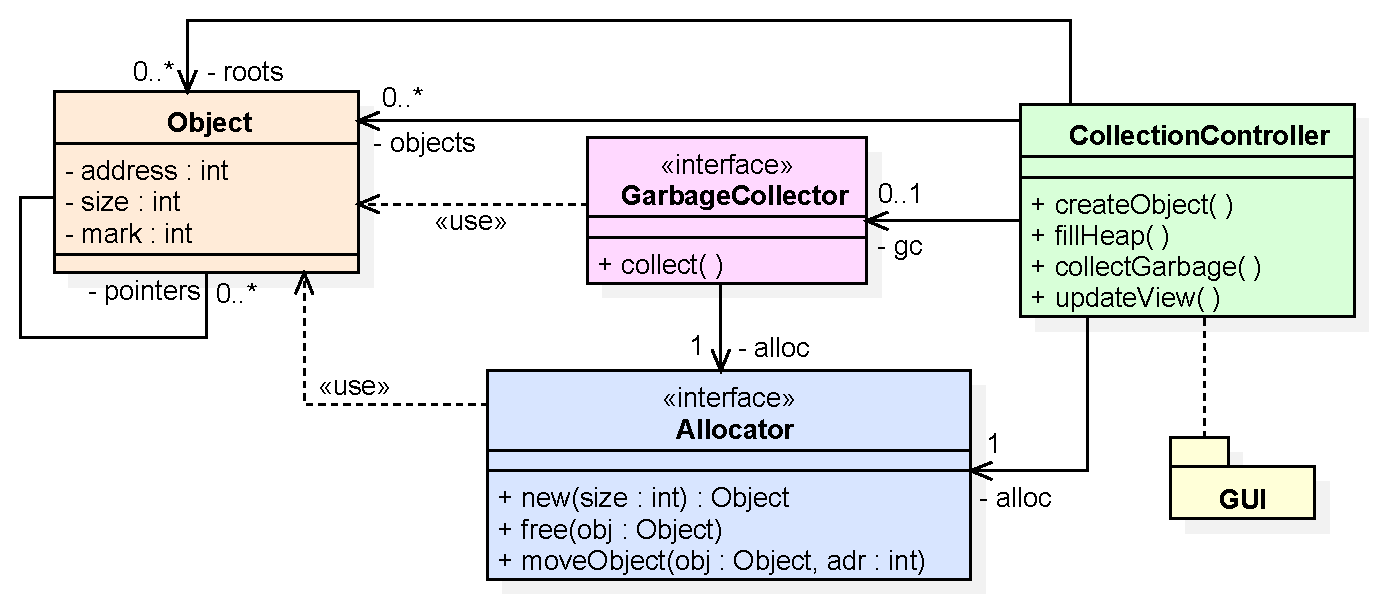
\includegraphics[scale=0.6]{img/uml/ch7-model.pdf}
	\caption[Klassendiagramm zur Modellierung von Mutator, Allokator, Kollektor]{Klassendiagramm zur Modellierung der Beziehung zwischen Mutator, Allokator und Kollektor. Im Rahmen der Implementation wurde dieses Modell um weitere Klassen, Methoden und Attribute ergänzt.}
	\label{fig:model}
\end{figure}

Heapobjekte werden als Instanzen einer Klasse \code{HeapObject} modelliert und beinhalten Speicheradresse (\code{address}), Größe (\code{size}), Markierungsinformation (\code{mark}) und eine Menge \code{pointers} an Referenzen auf weitere Instanzen von \code{HeapObject}, um die Menge \Pointers zu realisieren.
Ansonsten bieten sie keinerlei Funktionalität an.

Eine Instanz der Schnittstelle \code{Allocator} stellt die wesentlichen Dienste eines Allokators zur Verfügung.
Dazu zählt die Anforderung einer Speichermenge durch den Mutator mittels \code{new}, die Freigabe von Objekten und des durch sie belegten Speicherbereichs sowie das Verschieben eines Objekts.
Ersteres geschieht durch Übergabe der gewünschten Speichermenge und Rückgabe eines neu erzeugten Instanz von \code{HeapObject}, die die entsprechende Speicheradresse enthält.
Der Allokator ist diejenige Instanz, die Informationen über den Füllstand des Heaps und insbesondere über die Belegung einzelner Wörter besitzt.
Die abstrakte Klasse \code{GarbageCollector} beschreibt die Funktionalität eines Kollektors, welche im Wesentlichen aus der Durchführung eines Garbage-Collection-Zyklus (Methode \code{collect}) besteht.
Da eine Garbage Collection die Freigabe und Verschiebung von Objekten auslösen kann, benötigt sie die entsprechende Funktionalität von \code{Allocator}.
Die Klasse \code{CollectionController} realisiert einerseits die Aufgabe des Mutators, das heißt die Anforderung von Speicher für neue Objekte sowie die (Simulation von) Referenzmanipulationen, die zur Verwaisung von Objekten führen.
Daher besitzt sie zwei Mengen von Heapobjekten \code{objects} und \code{roots}.
\code{objects} enthält dabei sämtliche Objekte des Heaps.
\code{roots} enthält jedoch -- im Gegensatz zur Menge \Roots\ -- keine Basisobjekte, sondern diejenigen Heapobjekte, die von Basisobjekten referenziert werden.
Basisobjekte selbst werden somit aus der Simulation fortgelassen.
Zudem verwaltet \code{CollectionController} eine \code{Allocator}-Instanz, um Speicher anfordern zu können, sowie eine \code{GarbageCollector}-Instanz zur Auslösung der Garbage Collection.
Letztere ist zudem in der Lage, über den \code{CollectionController} auf die beiden Objektmengen sowie den eingesetzten Allokator zuzugreifen.
Andererseits fungiert \code{CollectionController} als Steuerklasse, um über die GUI eingehende Benutzerinteraktionen umsetzen und delegieren zu können (siehe Abschnitt~\ref{sec:gui}).

Die Idee ist nun, beim Start des Simulators zunächst eine Instanz der Klasse \code{CollectionController} erzeugen.
Diese legt wiederum -- je nach ausgewählter Garbage Collection -- eine geeignete \code{Allocator}-Instanz sowie einen \code{GarbageCollector} an und trägt sich beim Garbage Collector als Steuerinstanz ein.
Dadurch greifen Kollektor, Allokator und Steuerklasse auf denselben simulierten Heap zu.

\section{Implementation zentraler Komponenten}
\label{sec:implementation}
Im nun folgenden Abschnitt wird vorgestellt, wie die obige Modellierung unter Beachtung der spezifizierten Anforderungen realisiert wird.
Dabei wird zunächst die Umsetzung des Speichermodells und der Programmlogik fokussiert.
Abschnitt~\ref{sec:gui} widmet sich anschließend der Anbindung an die grafische Benutzerschnittstelle.

Im Sinne der Plattformunabhängigkeit wird dazu die Programmiersprache \textit{Java} gewählt, wobei auf die \textit{Java Language Specification 9}\footnote{\url{https://docs.oracle.com/javase/specs/jls/se9/html/index.html}} zurückgegriffen wird.
Der gesamte Programmcode wird über das Versionskontrollsystem \textit{Git}\footnote{\url{https://git-scm.com/}} verwaltet.
Um eine plattformunabhängige Entwicklung zu gewährleisten, kommt zudem das Build-Management-Tool \textit{Apache Maven}\footnote{\url{https://maven.apache.org/}} zum Einsatz.
Dieses bildet die verschiedenen Arbeitsschritte der Entwicklung, wie etwa Kompilieren, Testen und Erzeugen von \code{JAR}-Dateien, auf automatisiert durchführbare Phasen ab und kümmert sich dabei eigenständig um Abhängigkeiten von externen Bibliotheken.
Zur Weiterentwicklung des Systems genügt somit ein Klonen des Git-Repositorys und eine Ausführung von Maven, um alle benötigten Abhängigkeiten beschaffen zu lassen.

Bei der Entwicklung der einzelnen Komponenten wird grundsätzlich \textit{testgetrieben} vorgegangen.
Das bedeutet, dass zu jeder zu implementierenden Methode zunächst mehrere Testfälle erstellt werden, die das erwartete Verhalten des Programms beschreiben.
Einzige Ausnahme bilden hier Methoden, die mit GUI-Komponenten interagieren, da diese nur schwer automatisiert testbar sind.
Als Testframework wird auf \textit{JUnit 5}\footnote{\url{https://junit.org/junit5/}} zurückgegriffen.

\subsection{Heapobjekte (\code{pst.gcsim.Objects})}
\label{sub:heapobject}
Die Implementation der Klasse \code{HeapObject} unterscheidet sich nur unwesentlich von der in Abschnitt~\ref{sec:model} aufgeführten Modellierung.
Erwähnenswert ist jedoch die zusätzlich implementierte Klasse \code{AddressComparator} (siehe \ref{java:comparator}):
Da es in manchen Zusammenhängen sinnvoll ist, Objektmengen sortieren zu können (siehe etwa Abschnitt~\ref{sub:impl-gc}), vergleicht diese \code{Comparator}-Implementation Objekte anhand ihrer Speicheradresse.
Damit zwei verschiedene Objekte mit gleicher Speicheradresse nicht fälschlicherweise als identisch eingestuft werden, werden sie im Zweifelsfall zusätzlich nach einer internen ID verglichen.\footnote{Die Java 9 API-Spezifikation der Klasse \code{Comparator} empfiehlt, dass für zwei Objekte \code{a} und \code{b} der Ausdruck \mintinline[fontsize=\footnotesize]{java}{compare(a,b)} genau dann zu \code{0} auswertet, wenn \mintinline[fontsize=\footnotesize]{java}{a.equals(b)} zu \mintinline[fontsize=\footnotesize]{java}{true} auswertet. Diese Bedingung ist etwa für sortierte Datenstrukturen wie \code{TreeSet} wichtig, die keine Duplikate zulassen und \code{compare} zur Überprüfung auf Gleichheit heranziehen.}
Diese ist ein zusätzliches Attribut, das beim Erstellen eines \code{HeapObject} vergeben wird.

\begin{listing}[h]
	\inputminted[]{java}{code/AddressComparator.java}
	\caption[Klasse \code{AddressComparator} zum Vergleich von Objekten]{Die Methode \code{compare} der Klasse \code{AddressComparator} vergleicht zwei Objekte anhand ihrer Speicheradresse.}
	\label{java:comparator}
\end{listing}

\begin{figure}[t!]
	\centering
	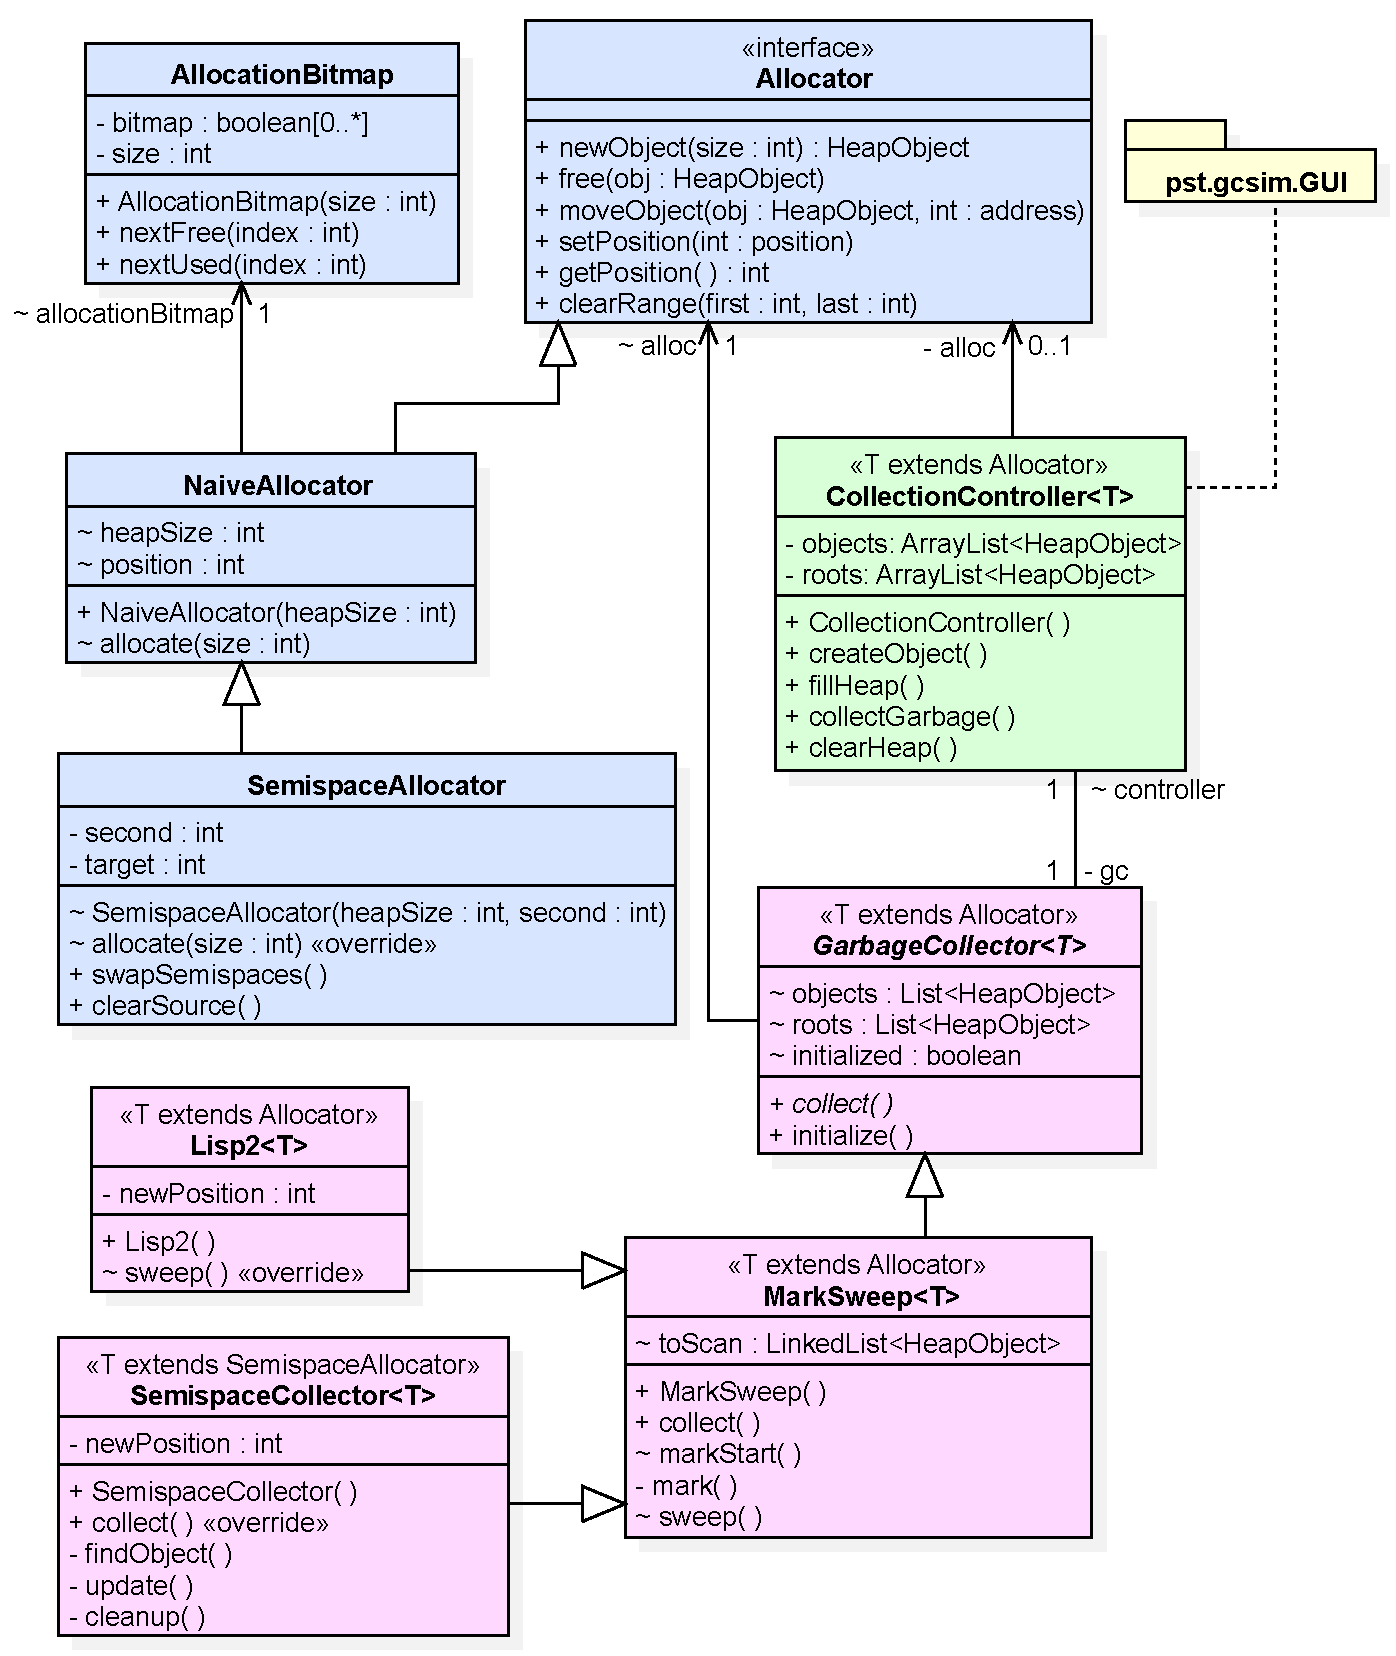
\includegraphics[scale=0.6]{img/uml/ch7-klassen.pdf}
	\caption[Klassendiagramm des realisierten Modells (Auszug)]{Klassendiagramm (Auszug) des realisierten Modells aus Abbildung~\ref{fig:model}.}
	\label{fig:implementation}
\end{figure}

\subsection{Allokatorklassen (\code{pst.gcsim.Allocators})}
\label{sub:allocator}
Der Allokator verwaltet die Information, welche Wörter des simulierten Heaps belegt sind.
Aus diesem Grund wurde zunächst eine Klasse \code{AllocationBitmap} entworfen, die diese Information in einem \mintinline{java}{boolean}-Array speichert (siehe Abbildung~\ref{fig:implementation}).
Der $i$-te Eintrag dieses Arrays gibt an, ob das $i$-te Wort des Heaps durch ein Objekt belegt (\mintinline{java}{true}) oder frei (\mintinline{java}{false}) ist.
Weiter stellt \code{AllocationBitmap} zwei Methoden \code{nextFree} und \code{nextUsed} zur Verfügung, welche ausgehend von einer übergebenen Speicheradresse die nächste freie bzw. belegte Stelle des Heaps liefern, indem das Array linear durchsucht wird.
Diese Methoden sind essenziell, um für eine angeforderte Speichermenge eine hinreichend große freie Stelle zu finden.

Als Konkretisierung der Schnittstelle \code{Allocator} wurde zunächst ein naiver Allokator entwickelt.
Dieser zeichnet sich dadurch aus, dass er -- ausgehend von einer Startposition -- mittels linearer Traversierung die nächstbeste freie Stelle findet, die die angeforderte Speichermenge aufnehmen kann.
Die Startposition ist dabei gegeben durch das Attribut \code{position}, welches stets die Adresse des ersten Worts hinter dem zuletzt angelegten Objekt enthält.

Das Herzstück der Klasse \code{NaiveAllocator} ist die Methode \code{allocate}, die intern durch \code{newObject} aufgerufen wird und das Auffinden einer geeigneten Position für ein neues Heapobjekt übernimmt (siehe Listing~\ref{java:naive-alloc}).
Diese Methode sucht zunächst unter Zuhilfenahme von \code{nextFree} und \code{nextUsed} der Reihe nach alle freien Stellen hinter \code{position} ab, bis eine genügend große gefunden oder das Ende des Heaps erreicht wurde (Zeile~7 bis~14).
Dabei wird auch berücksichtigt, dass sich hinter \code{position} eventuell kein freier Speicher befindet (Zeile~9f) oder ein freier Speicherbereich sich bis ans Heapende erstreckt (Zeile 12f).
Wird so ein hinreichend großer Bereich freien Speichers gefunden, wird dieser entsprechend der angeforderten Speichermenge als belegt markiert und die Anfangsadresse des Bereichs zurückgegeben (Zeile~18 bis 22).
Andernfalls wird auf analoge Weise der Bereich vor \code{position} durchsucht.
Sollte auch hierbei kein geeigneter Speicherbereich gefunden werden können, wird als Ergebnis \code{-1} zurückgegeben, was \code{newObject} dazu veranlasst, kein neues Objekt zu erzeugen.

\begin{listing}[h]
	\inputminted[]{java}{code/NaiveAlloc-allocate.java}
	\caption[Methode \code{allocate} der Klasse \code{NaiveAllocator}]{Auszug aus der Methode \code{allocate} der Klasse \code{NaiveAllocator}.}
	\label{java:naive-alloc}
\end{listing}

Der \code{SemispaceAllocator} wurde zur Realisierung des Halbraumverfahrens nach \textsc{Fenichel}, \textsc{Yochelson} und \textsc{Cheney} (siehe Abschnitt~\ref{sec:copying}) als Spezialisierung des naiven Allokators entwickelt.
Die Allokation läuft hier weitestgehend analog ab, allerdings wird der Allokationsversuch auf den aktuellen Zielhalbraum beschränkt, dessen Beginn im Attribut \code{target} notiert ist.
Zusätzlich steht eine Methode \code{swapSemispaces} zur Verfügung, die die Rolle der beiden Halbräume tauscht, sowie eine Methode \code{clearSource}, die einen Halbraum in Gänze als unbelegt markiert.

\subsection{Zentrale Steuerklasse \code{CollectionController}}
\label{sub:controller}
Die Klasse \code{CollectionController} verwaltet als zentrale Steuerklasse zum einen die beiden Objektmengen \code{objects} und \code{roots}, auf die von den implementierten Garbage-Collection-Algorithmen per Getter-Methoden zugegriffen werden kann.
Zum anderen bietet sie Methoden, um neue Objekte im Heap anzulegen bzw. bereits vorhandene Objekte verwaisen zu lassen.
Die Entscheidung, ob zwischen zwei Objekten eine Referenz erzeugt wird oder ein Objekt zur Menge der Basisobjekte gehört, wird dabei zufällig gefällt.
Die Wahrscheinlichkeit hierfür ist in der zentralen Konfigurationsklasse \code{Settings} (siehe Abschnitt~\ref{sub:settings}) hinterlegt und kann zur Laufzeit verändert werden.
Ebenso wird auch die Verwaisung eines Objekts simuliert (siehe Listing~\ref{java:controller-collect}):
Vor Auslösung der Garbage Collection wird zunächst über die Menge der Basisobjekte iteriert und bei jeder Iteration eine zufällige Zahl im Intervall $[0,1)$ bestimmt (Zeile~11).
Liegt diese unterhalb einer eingestellten Wahrscheinlichkeit, wird das Objekt aus der Menge der Basisobjekte entfernt.
Zur Vermeidung von Nebenläufigkeitskonflikten (\code{ConcurrentModificationException}), die bei Manipulation einer Datenstruktur auftreten, über die gleichzeitig iteriert wird, werden Löschkandidaten dabei zunächst zu einer separaten Liste hinzugefügt (Zeile~12).
Gleiches geschieht für jedes Objekt mit der Menge \code{pointers} der ausgehenden Referenzen.
Somit ist sichergestellt, dass jedes Objekt tatsächlich nach genügend Kollektionszyklen durch die Garbage Collection entsorgt wird, sofern die Verwaisungswahrscheinlichkeit größer als $0$ ist.

\begin{listing}[h]
	\inputminted[]{java}{code/Controller-collect.java}
	\caption[Methode \code{collectGarbage} der Klasse \code{CollectionController}]{Methode \code{collectGarbage} der Klasse \code{CollectionController}.}
	\label{java:controller-collect}
\end{listing}

Da die Steuerklasse den Garbage-Collection-Algorithmen den verwendeten Allokator zur Verfügung stellt, ist \code{CollectionController} als \textit{generische Klasse} konzipiert.
Der Typparameter \code{T} muss dabei die Schnittstelle \code{Allocator} implementieren.
Würde das Attribut \code{alloc} stattdessen lediglich als Instanz von \code{Allocator} deklariert werden, gäbe es für die implementierten Garbage-Collection-Algorithmen keine Möglichkeit, speziellere Allokatoren mit zusätzlichen Methoden anzufordern, da sie lediglich Zugriff auf die durch die Schnittstelle definierten Methoden hätten.
Aus gleichem Grund sind auch alle Kollektorklassen generisch, wobei jeder Kollektor zusätzliche Anforderungen an den Typparameter stellen kann.

\subsection{Kollektorklassen (\code{pst.gcsim.GarbageCollectors})}
\label{sub:impl-gc}
Die abstrakte Klasse \code{GarbageCollector} besitzt sämtliche Attribute und Methoden, die von allen konkret implementierten Garbage-Collection-Algorithmen verwendet werden.
Neben der Anbindung an den \code{CollectionController} gehört dazu auch eine Methode \code{isInitialized}, das angibt, ob eine Verbindung zur Steuerinstanz besteht.
Erst dann ist eine Auslösung der Garbage Collection möglich.

\begin{listing}[t!]
	\inputminted[]{java}{code/MarkSweep-core.java}
	\caption[Implementation der Drei-Farben-Abstraktion]{Implementation der Drei-Farben-Abstraktion in der Klasse \code{MarkSweep} (vgl. auch Algorithmus~\ref{algo:tricolor}).}
	\label{java:tricolor-core}
\end{listing}

Konkret wurden im Rahmen dieser Arbeit der Mark-Sweep-Algorithmus mit Drei-Farben-Abstraktion, die Lisp-2-Kompaktierung und die kopierende Garbage Collection implementiert.
Zunächst wurden die Algorithmen unabhängig von der geplanten grafischen Ausgabe umgesetzt.
Dieses Vorgehen hat den Vorteil, dass sich die vorgestellten Algorithmen auf recht kanonische Weise anhand ihrer Pseudocode-Beschreibung implementieren und anschließend testen lassen.
So weist etwa der Java-Code der \code{MarkSweep}-Klasse starke Ähnlichkeiten zum Pseudocode in Algorithmus~\ref{algo:tricolor} auf (siehe Listing~\ref{java:tricolor-core}).
Der einzige nennenswerte Unterschied ist die Umsetzung der linearen Heaptraversierung in der Bereinigungsphase:
Die implementierten Allokatoren besitzen zwar die Information, welche Bereiche des Heaps belegt sind, nicht aber, an welcher Adresse ein Objekt beginnt.
Daher wird die Traversierung simuliert, indem die Menge \code{objects} aller Heapobjekte vermöge des \code{AddressComparator}s nach den Adressen der Objekte sortiert und anschließend iteriert wird.
Auch hier landen Löschkandidaten zunächst in einer Liste \code{toRemove}, um \code{ConcurrentModificationException}s zu vermeiden.

\begin{listing}[t!]
	\inputminted[]{java}{code/Lisp2-core.java}
	\caption[Auszug der Klasse \code{Lisp2}]{Auszug der Klasse \code{Lisp2}, die als Spezialisierung von \code{MarkSweep} die \code{sweep}-Methode überschreibt.}
	\label{java:lisp2-core}
\end{listing}

Da sich die Markierungsphase des LISP-2-Algorithmus nicht von der des Mark-Sweep-Algorithmus unterscheidet (siehe Abschnitt~\ref{sec:lisp2-compact}), ist eine Spezialisierung der Klasse \code{MarkSweep} zur Umsetzung naheliegend.
In der Tat genügt es, in der Klasse lediglich die \code{sweep}-Methode zu überschreiben (siehe Listing~\ref{java:lisp2-core}).
Der große Unterschied zum Pseudocode-Algorithmus~\ref{algo:lisp2gc} ist allerdings -- neben der Simulation der linearen Traversierung -- der weitestgehende Verzicht auf die \code{update}-Methode:
Da die Verschiebung eines Objekts durch Manipulation des Attributs \code{address} bewerkstelligt wird, anstatt die Objekte tatsächlich im Speicher zu verschieben, ist hier eine Anpassung von Referenzen obsolet.
Das bedeutet gleichzeitig, dass dieser Schritt im Kollektionszyklus nicht mithilfe der entworfenen Modellierung dargestellt werden kann.
Die Kompaktierungsphase wird schließlich mit einer Freigabe des Heaps hinter den kompaktierten Bereich und einer Verschiebung der Allokatorposition ans Ende dieses Bereichs abgeschlossen (Zeile~17 bis 19), wodurch erneut zu sehen ist, dass beim Lisp-2-Algorithmus auf explizite Freigabe von Objekten verzichtet werden kann.
Allerdings muss jedes verwaiste Objekt mit Blick auf eine grafische Ausgabe aus \code{objects} entfernt werden, um auch aus der Menge aller Heapobjekte zu weichen.

Zuletzt sei ein Blick auf die Implementation des Halbraumverfahrens in der Klasse \code{SemispaceCollector} geworfen.
Auch hier zeigt sich zunächst eine deutliche Ähnlichkeit der Methode \code{collect} zum Pseudocode-Algorithmus~\ref{algo:copying-gc}, allerdings wird in der Methode \code{update} ebenfalls auf eine Anpassung von Referenzen verzichtet.
In Erinnerung daran, dass der ursprüngliche Algorithmus keine Objekte markiert, sondern unmittelbar bei Entdeckung in den anderen Halbraum verschiebt, fehlt somit zunächst die Möglichkeit zu erkennen, ob ein Objekt bereits kopiert wurde.
Zur Kompensation werden daher zusätzlich Markierungsinformationen genutzt, um zwischen unentdeckten, entdeckten (d.h. bereits kopierten) und fertig abgearbeiteten Objekten zu unterscheiden.
Dies hat den zusätzlichen Vorteil, diese drei Status in der grafischen Ausgabe optisch unterscheidbar machen zu können.
Auch beim Halbraumverfahren ist zuletzt eine Entfernung der verwaisten Objekte aus \code{objects} nötig, obschon der Quellhalbraum en bloc freigegeben werden kann.

\begin{listing}[h]
	\inputminted[]{java}{code/Semispace-core.java}
	\caption[Auszug der Klasse \code{SemispaceCollector}]{Auszug der Klasse \code{SemispaceCollector}. Im Gegensatz zum ursprünglichen Algorithmus~\ref{algo:copying-gc} wird zusätzlich die Markierungsinformation der Objekte genutzt.}
	\label{java:semispace-core}
\end{listing}

\subsection{Konfigurationsklasse \code{Settings}}
\label{sub:settings}
Die Konfigurationsklasse \code{Settings} enthält wesentliche Einstellungen zum Betrieb des Simulators sowie vorkonfigurierte Standardwerte (siehe Listing~\ref{java:settings}).
Dazu gehören etwa die Größe des Heaps (\code{HEAP\_COLS}, \code{HEAP\_ROWS}), die Größe erzeugter Objekte (\code{MIN\_OBJECT\_SIZE}, \code{MIN\_OBJECT\_SIZE}) und die Animationsgeschwindigkeit sowie Einstellungen, die Erreichbarkeit (\code{CONNECTIVITY}, \code{ROOT\_PROBABILITY}) und Verwaisung (\code{REFERENCE\_DELETION}) von Objekten beeinflussen.
Diese können über die grafische Oberfläche verändert werden (siehe Abschnitt~\ref{sec:execution}) und werden beim Beenden in einer Datei \code{gcsim.config} gesichert bzw. aus dieser geladen werden.
Zudem befindet sich in der Klasse \code{Settings} eine Auflistung der zur Verfügung stehenden Garbage-Collection-Algorithmen.
In Abschnitt \ref{sec:extension} wird erläutert, wie diese um weitere Algorithmen ergänzt werden kann.

\begin{listing}[h]
	\inputminted[]{java}{code/Settings.java}
	\caption[Auszug aus der Konfigurationsklasse \code{Settings}]{Auszug aus der Konfigurationsklasse \code{Settings}.}
	\label{java:settings}
\end{listing}

\section{Grafische Benutzerschnittstelle}
\label{sec:gui}
Für die Umsetzung der grafischen Benutzerschnittstelle wird auf das Framework \textit{Swing} sowie das \textit{Abstract Window Toolkit} (AWT) zurückgegriffen, die sich für die Entwicklung plattformunahängiger Oberflächen eignen.
Jedes Fenster wird dabei in einer eigenen Klasse umgesetzt (siehe Abbildung~\ref{fig:gui}).
Sogenannte \textit{Event Listener}, die auf Benutzerinteraktionen wie Button-Klicks, Textfeldeingaben und Fensterschließungen reagieren, werden dabei konsequent durch innere Klassen
realisiert.

\begin{figure}[h]
	\centering
	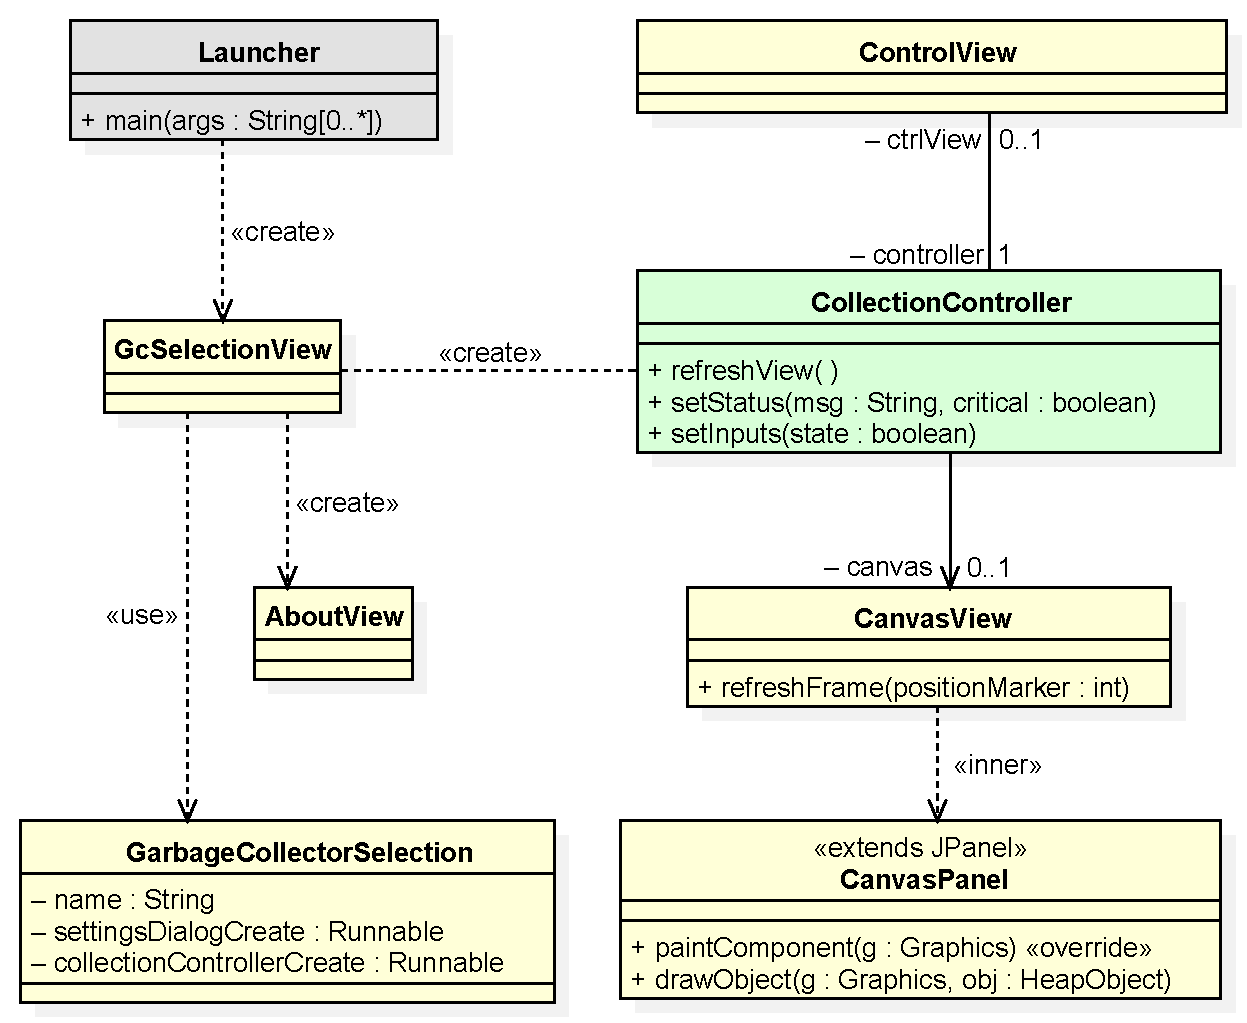
\includegraphics[scale=0.6]{img/uml/ch7-gui.pdf}
	\caption[Klassendiagramm des Pakets \code{pst.gcsim.GUI}]{Klassendiagramm (Auszug) des Pakets \code{pst.gcsim.GUI}. Zur Bedeutung der Klasse \code{GarbageCollectorSelection} siehe Abschnitt~\ref{sec:extension}.}
	\label{fig:gui}
\end{figure}

Das Herzstück der grafischen Ausgabe des Heaps bildet die Klasse \code{CanvasView}.
Diese besitzt neben einer Referenz auf die Menge \code{objects} der Steuerklasse und der aktuellen Position des Allokators zusätzlich die innere Klasse \code{CanvasPanel} als Spezialisierung der Swing-Komponente \code{JPanel} (siehe Listing~\ref{java:canvas}).
Durch Überschreibung der \code{paintComponent}-Methode können benutzerdefinierte Zeichnungen ausgegeben werden.
Diese Methode wird zum Rendern des Fensterinhalts aufgerufen, beispielsweise wenn das Fenster über den Bildschirmrand hinausgeschoben wird.
Ein manueller Aufruf durch den \code{CollectionController} ist über die Methode \code{refreshFrame} (Zeile~2 bis~6) möglich.

\begin{listing}[p]
	\inputminted[]{java}{code/CanvasView.java}
	\caption[Auszug aus der Klasse \code{CanvasView}]{Auszug aus der Klasse \code{CanvasView}. Zu sehen sind die Methoden \code{paintComponent} und \code{drawObject}, welche die grafische Ausgabe erzeugen.}
	\label{java:canvas}
\end{listing}

Da der Heap als zweidimensionale Grafik angezeigt werden soll, wird in der Methode \code{drawObject} zunächst anhand der Adresse des Heapobjekts \code{obj} die Startposition bestimmt (Zeile~22f).
Zudem wird anhand der Markierung die verwendete Farbe festgelegt (Zeile~26 bis~34).
Anschließend wird durch die \mintinline{java}{while}-Schleife das Objekt Zeile für Zeile gezeichnet (Zeile 37 bis 42).
Dadurch wird berücksichtigt, dass sich das Objekt gegebenenfalls über mehrere Zeilen erstreckt.
Zuletzt werden Linien gezeichnet, die Beginn und Ende des Objekts markieren.
Ein Objekt erscheint somit als farbiges, geschlossenes Rechteck mit eventuellen Zeilenumbrüchen.

Zum Schluss gehen wir darauf ein, wie im entworfenen Simulator die Ausführung der Garbage-Collection-Algorithmen umgesetzt wird.
Als nützliches Hilfsmittel hat sich hierfür die \code{Timer}-Komponente von Swing erwiesen.
Mittels eines Swing-Timers kann eine Reihe von Anweisungen periodisch in einem eigenen Thread ausführt werden, wobei der zeitliche Abstand zwischen zwei Ausführungen definiert werden kann.
Die Syntax dafür lautet wie folgt:

\vspace*{-0.5cm}
\begin{center}
	\mintinline{java}{new Timer(<Verzögerung>, <Parametername> -> <Anweisungsblock>);}
\end{center}

\vspace*{-0.5cm}
Dabei gibt der erste Parameter \code{<Verzögerung>} die Zeitspanne an, nach der die nächste Ausführung von \code{<Anweisungsblock>} ausgelöst wird.\footnote{Standardmäßig findet jedoch die nächste Ausführung nicht vor Beendigung der vorigen statt, sodass sich zwei Ausführungszyklen nicht überlappen. Für Details sei hier auf die API-Spezifikation von \code{javax.swing.Timer} verwiesen.}
Durch den Lambda-Ausdruck \code{<Parametername> -> <Anweisungsblock>} wird hier ad hoc ein \code{ActionListener} definiert.
Am Beispiel der Klasse \code{MarkSweep} lässt sich exemplarisch betrachten, wie ein derartiger Timer als Attribut in die Garbage-Collection-Algorithmen integriert werden kann (siehe Listing~\ref{java:mark-timed}):
Hier bietet es sich etwa an, mit jeder Timer-Auslösung das nächste Objekt aus \code{roots} zu markieren, sodass die Anwenderin sieht, wie nacheinander alle Basisobjekte markiert werden.
Demzufolge wird die ursprüngliche \mintinline{java}{for}-Schleife der Methode \code{markStart} unter Zuhilfenahme eines Iterators der Menge \code{roots} in den Anweisungsblock von \code{gcTimer} integriert (Zeile~7 bis~13).
Zusätzlich wird dabei die grafische Ausgabe des Heaps aktualisiert, um die erfolgte Markierung sichtbar zu machen (Zeile~12).
Nachdem der Timer definiert wurde, wird er gestartet (Zeile~19).
Sobald alle Basisobjekte abgearbeitet wurden, ist die Bedingung in Zeile~7 nicht mehr erfüllt, sodass sich der Timer im \mintinline{java}{else}-Block selbst anhält und die Methode \code{markTimed} aufruft.
In dieser wird \code{gcTimer} analog so definiert, dass mit jeder Iteration ein Objekt der Menge \code{toScan} abgearbeitet wird, sodass auch hier die Behandlung jedes einzelnen Objekts beobachtet werden kann.

\begin{listing}[h]
	\inputminted[lastline=20]{java}{code/MarkSweep-timed.java}
	\caption[Ausführung des Mark-Sweep-Algorithmus mithilfe eines Swing-Timers]{Ausführung des Mark-Sweep-Algorithmus mithilfe eines Swing-Timers. Mit jeder Auslösung des Timers wird ein weiteres Basisobjekt abgearbeitet. Im Anschluss an diese Phase wird der Timer angehalten und die Methode \code{markTimed} ausgeführt, in der \code{gcTimer} neu definiert und wieder gestartet wird.}
	\label{java:mark-timed}
\end{listing}

Der Vorteil von Swing-Timern ist die nebenläufige Ausführung des Anweisungsblocks in einem eigenen Thread:
Während ein Timer aktiv ist, wird dadurch der Rest der Anwendung nicht blockiert, sodass weiterhin Benutzereingaben möglich sind und die Animation der grafischen Ausgabe überhaupt sichtbar ist.
Dies ermöglicht zudem, den Timer anzuhalten und einen Algorithmus zu unterbrechen.
Offensichtlicher Nachteil ist die Integration in bereits implementierte Algorithmen, die im Zweifelsfall wenig intuitiv und fehlerträchtig ist.
Zwar lassen sich die mit Timern versehenen Algorithmen ebenfalls mit JUnit testen, allerdings müssen die Tests künstlich verzögert werden, da andernfalls Ergebnisse überprüft werden, bevor die nebenläufige Ausführung beendet wurde.